\documentclass[12pt]{article}
\usepackage[utf8]{inputenc}
% Language setting
% Replace `english' with e.g. `spanish' to change the document language
\usepackage[english]{babel}
\usepackage[T1]{fontenc}
% Set page size and margins
% Replace `letterpaper' with`a4paper' for UK/EU standard size
\usepackage[letterpaper,top=2cm,bottom=2cm,left=2cm,right=2cm,marginparwidth=1.75cm]{geometry}

\usepackage{colortbl}
\usepackage{wrapfig}
\usepackage{caption}
\usepackage{subcaption}
\usepackage[export]{adjustbox}
\usepackage{comment}

\usepackage[colorlinks=true, allcolors=blue]{hyperref}

%BIBLIO
\usepackage[backend=biber, style=numeric, sorting=none]{biblatex}
\addbibresource{Biblio_Rapport.bib}
\usepackage{wallpaper}

\usepackage{pict2e}
\setlength{\unitlength}{1mm}

%MATHS
\usepackage{mathtools}
\usepackage{amsmath}
\usepackage{amsfonts}
\usepackage{amssymb}
% Useful packages

\usepackage{graphicx}   %images
\usepackage{wrapfig}
\usepackage[colorlinks=true, allcolors=blue]{hyperref}  %mets les liens en couleur (ici bleue)
%\usepackage{pdfpages} %possibilité d'inclure de pdf
%\usepackage{float}
\usepackage{pdfpages} %inclure des fichiers pdf
\usepackage{listings} %insérer du code
\def\svgwidth{0.5\textwidth}%définit la taille des figures


\usepackage{geometry}
\usepackage{hyperref}

\usepackage{tikz}
\usetikzlibrary{shapes}
\usepackage{pgfplots}
\usetikzlibrary{plotmarks}
\pgfplotsset{compat=1.15}%ligne que je ne comprends pas trop
\usepackage{multicol}


\begin{document}


\begin{titlepage}
    \centering
    
    % Logos côte à côte
    
\includegraphics[width=0.4\textwidth, valign=c]{Logos/Logo_UT3.png} \hfill
    
\includegraphics[width=0.4\textwidth, valign=c]{Logos/EPFL.png}\par
    \vspace{2cm}

     \LARGE Internship report \par

    \vspace{2cm}

    {\Large \textit{04/08/2024 - 06/10/2024}}
    \vspace{1cm}
    
    % Titre du rapport de stage
    \hrule
    \vspace{0.5cm}
    \Huge \textbf{Shape effects on magnetic field fluctuations in TCV tokamak}
    \vspace{0.5cm}
    \hrule
    \vspace{3cm}

    % Informations sur l'auteur et l'encadrant
    \begin{minipage}[t]{0.45\textwidth}
        \raggedright
        \large
        \textbf{Author:}\\
        Gaëtan RÉGNIER\\
    \end{minipage}
    \hfill
    \begin{minipage}[t]{0.45\textwidth}
        \raggedleft
        \large
        \textbf{Supervisor:}\\
        Dr. Benoît LABIT\\
        Swiss Plasma Center\\
        benoit.labit@epfl.ch\\
    \end{minipage}\par
    
    
    \vfill
    
    % Pied de page avec le nom de la formation
    {\large L3 PHYSIQUE PARCOURS SPÉCIAL}\par
\end{titlepage}
\thispagestyle{empty}
\begin{abstract}
    
\end{abstract}

\tableofcontents
\newpage
\setcounter{page}{1}
\section{Introduction}

\subsection{Nuclear fusion and TCV}

\paragraph{}
Nowadays, the most efficient way that we know to produce energy is Nuclear Fission. It is probably one of the future most efficient and safest energy source. Nevertheless, we are not able to produce energy thanks to this process. Research about nuclear fusion represents a major concern for next years, and Swiss Plasma Center is a major actor of fusion research with its \textit{Tokamak à Configuration Variable} (also called TCV).
    
\subsubsection{What is Nuclear Fusion ?}

\paragraph{}
Nuclear fusion is the kind of nuclear reaction that occurs in the core of stars. In the future, it could become a nearly inexhaustible, low-carbonised and extremely safe energy source. Indeed, raw materials that we need are two isotopes of hydrogen : Deuterium \(_1 ^2 D\) and Tritium \(_1 ^3 T\). Deuterium is naturally present in water and represents 1/6500 molecules. With nuclear fusion, we would have enough deuterium to produce electricity for millions of years. Tritium does not naturally exists but it is possible to create it thanks to lithium which is also quite enough abundant to produce energy for tens of thousands of years \cite{yves_martin_fusion_2014}. There are several fusion reaction that exist but only one is considered to produce energy today because it has the highest success probability :

\begin{gather}\label{eq:Reaction D-T}
    _1 ^2 \textrm{D} + _1 ^3 \textrm{T} \rightarrow _2 ^4 \textrm{He} ~(3.50 \textrm{MeV}) + _0 ^1 \textrm{n}~(14.1 \textrm{MeV})
\end{gather}

\paragraph{}
Equation \ref{eq:Reaction D-T} shows that the fusion reaction produces the most common and stable helium isotope and a neutron with respectively 3.50 MeV and 14.1 MeV of kinetic energy \cite{holger_reimerdes_mhd_2001}. It could be also interesting to notice that there is not any radioactive waste or greenhouse gas produces. Finally, this equation shows that fusion reactions cannot imply chain reactions unlike nuclear fission which make it extremely safe. 

\subsubsection{Magnetic confinement and tokamak}

\paragraph{}
To make fusion happen, we need to overcome the Coulomb force which is in inverse proportion to distance between atoms. Thus we need to increase a lot kinetic energy to reach a temperature of about \(10^8\) °C \cite{yves_martin_fusion_2014}. When we reach those temperature, kinetic energy of atoms is sufficient to be fully ionised, this is the form of plasma. Thus, particles each particle has an electrical charge of \(\pm e\) which allows to confine it with magnetic field. Indeed, to maintain such a high temperature, we need to isolate plasma in a vacuum chamber. 

\paragraph{}
Moreover, it is important to reduce as much as possible contact between plasma and vacuum vessel. Is is possible thanks to a magnetic confinement which consists in applying firstly a toroidal magnetic field (magnetic field lines are circles of z axis) thanks to coils. Nevertheless as a toroidal field is not homogeneous, electrical charges are separated so it is important to add a poloidal magnetic field obtained by adding in order to keep global neutrality of plasma (this configuration is showed in figure \ref{fig:magnetic confinement}).  The toroidal chamber with this specific coil configuration is called a \textbf{tokamak}. 

\begin{figure}
    \centering
    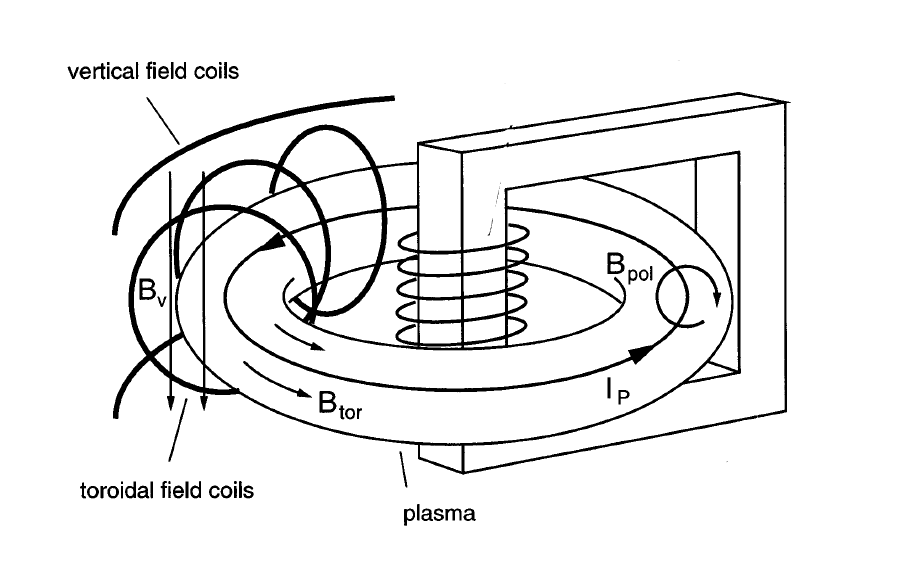
\includegraphics[scale=0.5]{Figures/Schéma confinement magnétique.png}
    \caption{Schématic of the coil configuration of tokamak. \(B_v\) is added in order to counter plasma pressure which tends to extand plasma by interacting with plasma current (\(d\Vec{F}=Idl(\Vec{e_{\phi}})\wedge B_v(-\Vec{e_z})=-dl I B_v \Vec{e_\rho}\)). \cite{holger_reimerdes_mhd_2001}}
    \label{fig:magnetic confinement}
\end{figure}


\subsubsection{TCV presentation}

\paragraph{}
I worked on data that were produced by TCV tokamak (\textit{Tokamak à Configuration Variable}) of Swiss Plasma Center in Lausanne, Switzerland. It is called like this because each coil is supplied individually which allows to study a lot of different plasma shapes. 

\subsection{Magnetic probes in TCV}

\subsubsection{Mirnov probes}\label{Mirnov Probes}

\paragraph{}
Mirnov probes are magnetic probes which aim is to measure poloidal magnetic field. There are 4 sets of 38 probes separated by 90° which are located in sectors 3, 7, 11 and 15. Each set of 38 probes can be separated into 3 arrays : "top", "middle" and "bottom" (cf figure \ref{fig:Mirnov Probes}). When we download data acquired by Mirnov probes, we can choose if we want data from one of three arrays or from all probes. 

\begin{figure}
    \centering
    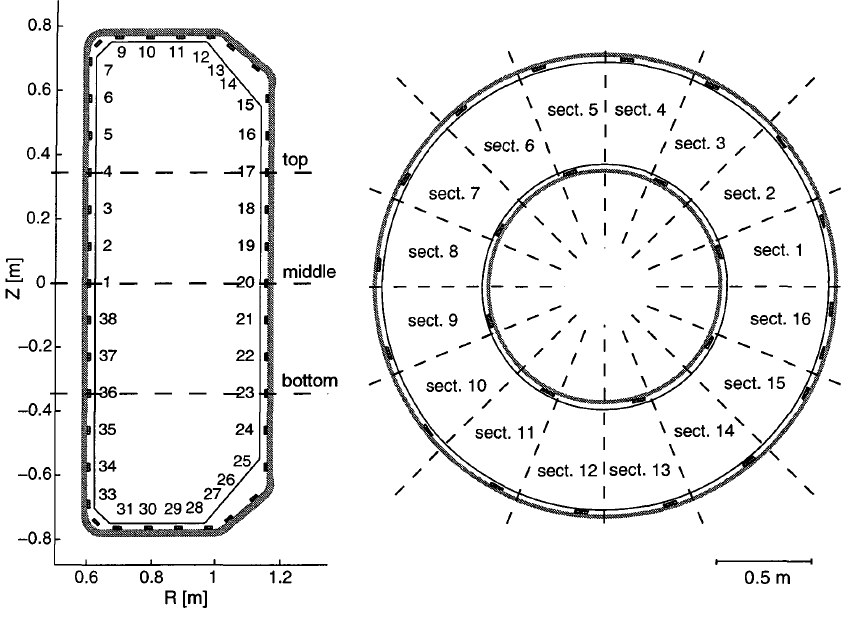
\includegraphics[scale=0.5]{Figures/Mirnov Probes arrangements.png}
    \caption{Arrangement of TCV Mirnov probes in different arrays (on the left) and tokamak sectors (on the right)\cite{holger_reimerdes_mhd_2001}}
    \label{fig:Mirnov Probes}
\end{figure}

\subsubsection{LTCC - 3D probes}

\paragraph{}
Low-Temperature Co-fired Ceramic 3D (LTCC-3D) probes are able to measure each components of magnetic field. Actually, those probes measures magnetic field fluctuations \(\delta B / \delta t\) on three components : vertical, radial and toroidal components. Then, it is possible to integrate acquired data to get the three components of magnetic field \( B_z, B_{rad} \) and \( B_{tor}\) \cite{duccio_testa_manufacturing_2020}. 

\paragraph{}
They are located inside the TCV vacuum vessel and there are three LTCC-3D probes. The sampling frequency of LTCC-3D probes is of 2 MHz which means that Nyquist frequency (highest frequency measurable obtained by Shannon's law) associated to those probes is 1 MHz which is quite more that Mirnov probes mentioned in section \ref{Mirnov Probes}. Figure \ref{fig:???} shows the different spectrograms of signal acquired respectively by Mirnov Probes and LTCC-3D probes. 



\subsection{How to produce energy with nuclear fusion ?}

\subsubsection{Conditions}

\subsubsection{Magnetic confinment}

\subsubsection{Issues encountered}

\paragraph{}
To reach the highest probability of success of nuclear fusion reaction, the temperature have to be around 100 million degrees in the core of plasma. Whereas, this huge temperature implies a lot of instabilities. Indeed, the value called \textbf{plasma parameter} verifies (with density \(n \sim 10^{19} \textrm{ m}^{-3}\)) : 

\begin{equation}
    \Xi \approx 10^{-5} \left (\frac{n}{10^{12}}\right)^{1/3} \left(\frac{T}{10^6}\right)^{-1}
\end{equation}

And when \(\Xi \ll 1\), plasma is called \textbf{kinetic plasma} and this kind of plasma is subject to a lot of instabilities because of disorder \cite{antoine_strugarek_turubulence_2012}. Thus, tokamaks plasmas are always kinetic ones because of the huge temperature which is about \(10^8\) K. The heat of the core of plasma tends to be evacuated outside which creates a heat flux, an instabilities source. In order to produce energy later thanks to nuclear fusion, it is crucial to be able to minimize this flux which is called \textbf{transport} to keep as much energy as possible in order to limit energy loss by confining it in the core of plasma. 

\paragraph{TEMPS DE CONFINEMENT}
The quality of confinement can be materialised by \textbf{confinement time} which is equal to total plasma energy over power loss (or power that we have to inject to keep a constant energy in stationnary regime) :

\begin{equation}
    \tau_E = \frac{E_{tot}}{P_{loss}}
\end{equation}

\subsection{Flux surfaces and plasma shape}

\paragraph{FLUX SURFACES}

\paragraph{}
Plasma shape is determined by the last closed flux surface which can be mostly described by two main parameters : \textbf{elongation} written \(\kappa\) and \textbf{triangularity} written \(\delta\). 

\begin{figure}
    \centering 
    \input{dessin_élongation_triangularité.pdf_tex}
    \caption{Representation of last closed flux surface with useful distances}
    \label{fig:determinaton kappa&delta}
\end{figure}

\paragraph{}
Elongation is the quotient between plasma length and plasma width (\(b/a\) on the right side of figure \ref{fig:determinaton kappa&delta}). Triangularity is the quotient between abscissa of the lowest (or highest) point of the last closed flux surface and half of plasma width (\(d/a\) on the right side of figure \ref{fig:determinaton kappa&delta}). It can be interesting to notice that \textit{d} is an algebric distance. Thus, triangularity can be positive or negative. On the right side of figure \ref{fig:determinaton kappa&delta}, \(d>0\) so \(\delta >0\). A difference can also be made between \(\delta_{bot}\) and \(\delta_{top}\), they respectively take in account the bottom and the top of last closed flux surface to measure \(d\) on the figure \ref{fig:determinaton kappa&delta}. \(\delta\) is the mean of \(delta_{top}\) and \(\delta_{bot}\). In TCV, \(\kappa\) and \(\delta\) verify : \(1 \leq \kappa \leq 2.8\) and \(-0.8 \leq \delta \leq 0.9\).



\subsection{Consequences of negative triangularity on transport and confinement time}

\paragraph{}
In \cite{yann_camenen_etude_2006}, it has been showed that plasmas with \(\delta < 0\), electronic thermal energy transport was significatively decreased instead of plasmas with \(\delta > 0\) for equivalent experimental parameters. Moreover, this paper verified experimentally the empirical law found in \cite{A_Pochelon_1999} for plasmas that will be studied in this report :

\begin{equation}
    \tau_{Ee} \propto (1+\delta)^{-0.35}
\end{equation}

\paragraph{}
It shows that electronic confinement increases when \(\delta\) decreases which means that transport is reduced. That the focus is made here on plasmas with negative triangularity. 





\section{Methods}

\subsection{MDB database}

\paragraph{}
MDB is a database software that have been developed specifically to manage TCV data. It can be  considered as a table where different variables describing parameters that we choose. In concrete terms, some specific variables named \textbf{key variables} are used to identify a specific shot and the time interval that we want to analyse. For instance, key variables that we chose were the \textbf{shot number} (noted SHOT), the middle \textbf{time} (noted TIME) of the analysed interval and the \textbf{duration} (noted MDBTSM) of the interval analysed. Then, other variables can be stored in database as plasma current, triangularity, elongation, power heating...

\begin{table}[h]
    \centering
    \begin{tabular}{|c|c|c|c|c|c|c|}
        \hline
        \multicolumn{3}{|c|}{key variables} & \multicolumn{4}{|c|}{}\\
        \hline
        SHOT & TIME & MDBTSM & KAPPA & DELTA & POHM & IP \\
        \hline
        69085 & 0.65 & 0.2 & 1.33 & -0.32  & \(2.43.10^5\) & \(-2.32.10^5\) \\
        69088 & 1.2 & 0.2 & 1.32 & 0.12 & \(4.84.10^4\) & \(-1.22.10^5\) \\
        69092 & 0.3 & 0.1 & 1.63 & 0.09 & \(1.55.10^5\) & \(1.78.10^5\) \\
        69108 & 0.75 & 0.2 & 1.50 & -0.28 & \(2.58.10^5\) & \(2.16.10^5\) \\
         \hline
         
    \end{tabular}
    \caption{Simple MDB database example}
    \label{tab:mdb example}
\end{table}

\paragraph{}
It is important to notice that there are no units in MDB database, so we must be aware about the fact that data collected has to be in International System units. 

\paragraph{}
Actually, data is stored in a MATLAB file (.MAT) as a structure. A MATLAB structure is an array of different vectors that can be called by their name. If the name of the structure is \texttt{data}, the vector \texttt{data.KAPPA} contains elongation of all samples (one sample corresponding to an index). For instance here, \texttt{data.SHOT(1) = 69085}. Each value collected is meaned on the interval analysed.

\paragraph{}
To collect data, MDB uses two different files, an MDB file (.mdb) in which we can write the label of each variable, the interval analysed, the method used to collect it and if it is required, the expression needed. For example, it is possible to use MATLAB method, which means that data is collected thanks to a MATLAB or a MATLAB routine. The second file used is the MAN file (.man) in which we must write (manually) the value of keys variables. Extracts of MDB file and MAN file are showed in the figures \ref{fig:mdb file} and \ref{fig:man file}.



\begin{figure}[h]
    \begin{minipage}{0.5\textwidth}
        \centering
        %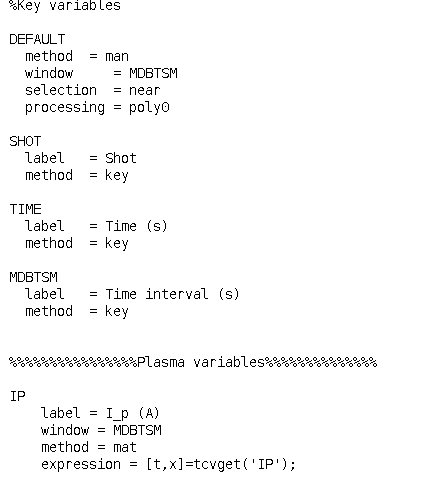
\includegraphics[width=0.8\textwidth]{Figures/MDB file.png}
        \begin{lstlisting}
        %Key variables
        SHOT
            label   = Shot
             method  = key

        TIME
             label   = Time (s)
            method  = key

        MDBTSM
            label   = Duration (s)
            method  = key

        %Plasma variables

        IP
            label = I_p (A)
            window = MDBTSM
            method = mat
            expression = [t,x]=tcvget('IP');
        \end{lstlisting}
        \caption{Extract of MDB file. Here, "mat" corresponds to matlab method, so data is collected thanks to a matlab function}
        \label{fig:mdb file}
    \end{minipage}
    \begin{minipage}{0.5\textwidth}
        \centering
        %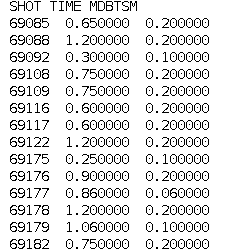
\includegraphics[width=0.8\textwidth]{Figures/MAN file.png}
        \begin{lstlisting}
        SHOT TIME MDBTSM
        69117  0.600000  0.200000
        69122  1.200000  0.200000
        69175  0.250000  0.100000
        69176  0.900000  0.200000
        69177  0.860000  0.060000
        69178  1.200000  0.200000
        69179  1.060000  0.100000
        69182  0.750000  0.200000
        69196  0.500000  0.200000
        69196  1.600000  0.200000
        69200  0.320000  0.050000
        69201  0.800000  0.200000
        69203  0.300000  0.050000
        69207  0.600000  0.200000
        69207  0.870000  0.100000
        69207  1.100000  0.140000
        69207  1.350000  0.100000
        69207  1.600000  0.140000
        69208  0.500000  0.140000
        69208  0.850000  0.140000
        69208  1.100000  0.200000
        \end{lstlisting}
        \caption{Extract of MAN file}
        \label{fig:man file}
    \end{minipage}
\end{figure}

\subsection{Sample selection}

\paragraph{}
In MDB database, each value of the data file (that can be considered as a similar object than table \ref{tab:mdb example}) is meaned on the time interval that has been selected. That is why it is important to consider only time intervals where shape parameters are constants (or can be assumed as constants). But selection will be more understandable if we look at an example of selection. First of all, the summary of most important data related to a shot can be compiled in a scope that we can see on figure \ref{fig:jScope shot summary}.

\begin{figure}[h]
    \centering
    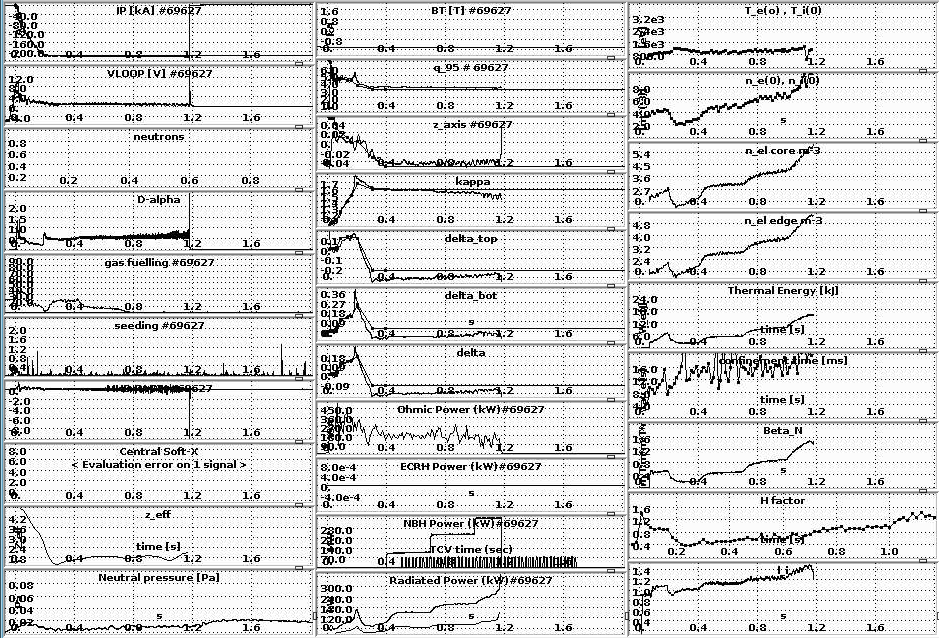
\includegraphics[width=0.8\textwidth]{Figures/shot_summary_69627.png}
    \caption{Summary of shot n° 69627}
    \label{fig:jScope shot summary}
\end{figure}

\paragraph{}
Figure \ref{fig:jScope shot summary} is a good example to explain sample selection. Indeed, three main time intervals can be interesting in this only shot. NBH power is constant on three different intervals after plasma setting up : approximately from 0.4 sec to 0.7 sec, from 0.7 sec to 1.0 sec and from 1.0 to 1.17 sec (corresponding to disruption). In those intervals, we are looking for shorter time intervals where all plasma shape parameters can be assumed as constants (plasma current, gas fuelling, \(\delta\), \(\kappa\), density (\(n\)), \(\beta\), magnetic axis coordinates\dots). In 1.0-1.17 sec time interval, density is variating too much to be considered as constant. That is why, we chose to not use this one. We chose to keep 0.44-0.76 sec interval and 0.85-1.05 sec time interval. 

\subsection{Variables selection}

\paragraph{}
Now that we know which sample to analyse, we have to do a variable selection. Indeed, to see if a plasma shape parameter influences magnetic field, we firstly has to select variables that are not correlated together. For instance, area of plasma section is intrinsically correlated to plasma volume and that is why it is not really relevant to look at impact of both variables on magnetic field. The idea is now to etablish a list of variables as less correlated as possible and describing well all plasmas parameters. The first step to do it is to take in account a great amount of variables that could potentially affects magnetic field. Then, correlation between all of those variables will be showed thanks to a correlation table. 



\paragraph{PYTHON PROGRAM, méthode pearson}
 
\appendix

%\newpage
\section{Synthèse de cours du traitement du signal}

\subsection{Reminder on Nyquist-Shannon Theorem}

\paragraph{Theorem :}
A continuous-time signal of finite bandwidth, that has been
sampled, can be perfectly reconstructed from a finite sequence of
samples if the sampling rate exceeds 2F samples per seconds, F being
the highest frequency of the original signal.

\paragraph{}
There are two cases to consider here : 

If the highest frequency of the signal is known and equal to \(f\), we need a sampling frequency superior to \(2f\) to describe it correctly. The frequency \(2f\) is called the \textbf{Nyquist rate}.

Whereas, if only the sampling frequency is known as \(f_S\), it means that the highest frequency of the have to be inferior to \(f_S/2\). The frequency \(f_S / 2\) is called the \textbf{Nyquist frequency} noted here \(f_N\). 

\paragraph{}
If those conditions are not satisfied, aliasing phenomenon can be observed. It means that is the highest frequency of the signal is noted \(f_1\) and \(f_1 > f_N\), the frequency observed is \(f = f_S - f_1\).

\paragraph{}
To avoid it, there are two main possibilities, the first one that can be the most intuitive which is to increase the sampling frequency. Nevertheless, it also possible to use an anti-aliasing filter. It is basically a high-pass filter so it can implies to lose some frequencies in the signal but at least, it is a good tool to be certain that there are no false frequencies measured.


\subsection{Discrete Fourier Transform}

\paragraph{}
The Discrete Fourier Transform (or DFT) is a good way to approach the real value of Fourier Transform by a numerical way, if we consider \(x_j\) \(1 \leq j \leq N\) all the samples of signal separed by a duration \(\Delta t = \frac{1}{f_S}\) and \(X_k\) coefficients referred to the signal spectrum, they verify the relations : 

\begin{gather}
    X_k = \sum_{j=0}^{N-1} x_j e^{2i\pi \frac{j k}{N}} ~~~~~~k=0,\dots,N-1 \\
    x_j = \frac{1}{N}\sum_{k=0}^{N-1} X_k e^{2i\pi \frac{j k}{N}} ~~~~~~ j=0,\dots, N-1
\end{gather}

\subsubsection{Units}

\begin{figure}[h]
    \begin{minipage}{0.5\textwidth}
        Spectral resolution :
    \begin{equation*}
    \Delta f = \frac{f_S}{N}
    \end{equation*}

    Frequency range :
    \begin{equation*}
        f=\left[- \frac{N}{2} +1 ; \frac{N}{2} \right]
    \end{equation*}
    \end{minipage}
    \begin{minipage}{0.5\textwidth}
    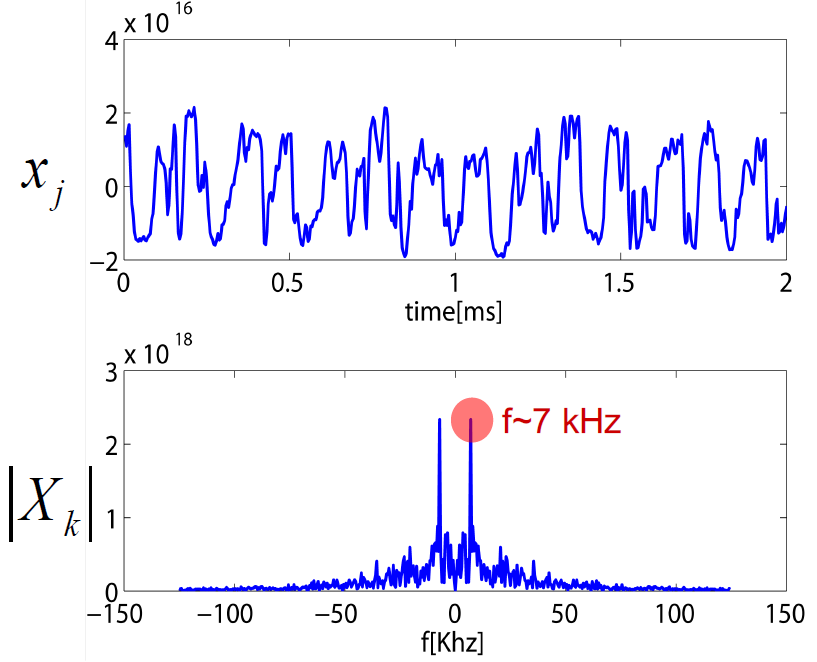
\includegraphics[scale=0.4]{Figures Cours Traitement du Signal/Units of DFT.png}
    \caption{A signal and its DFT}
    \label{fig:DFT example}
    \end{minipage}
\end{figure}

\newpage
\subsubsection{Time-frequency representation : the spectrogram}

One thing that we can notice with the representation of figure \ref{fig:DFT example} is that when DFT (or a classical Fourier Transform) is applied to a signal, we totally lose the information of time. To keep both informations (frequency and time), we use a matrix that is called a spectrogram which allows to represent both. 

\begin{figure}[h]
\begin{minipage}{0.4\textwidth}
    Coefficients of corresponding matrix are are given by : 

    \begin{equation*}
        S_{n,k}=\Delta t \sum_{j=(n-1)M} ^{nM} x_j e^{+2\pi i \frac{j k}{M}}
    \end{equation*}
    With \(1\leq M \leq N\)

    \paragraph{}
    It is a \(N \times (N/M)\) matrix 
\end{minipage}
\begin{minipage}{0.6\textwidth}
\centering
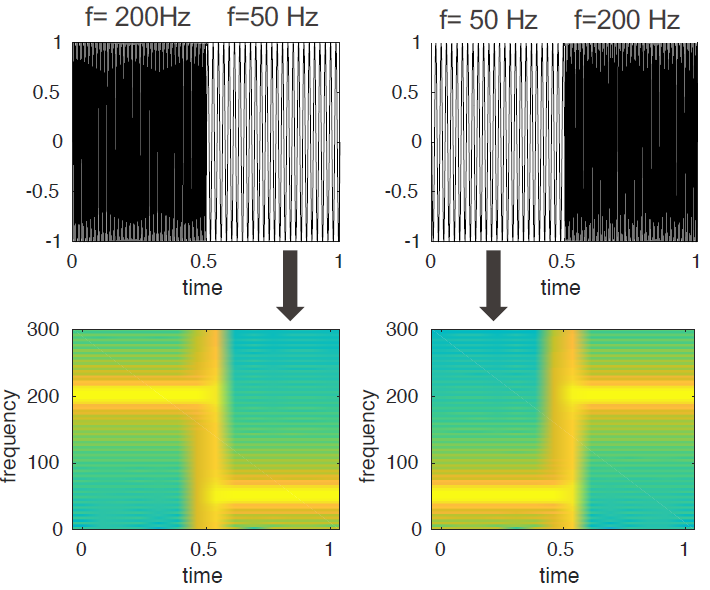
\includegraphics[scale=0.5]{Figures Cours Traitement du Signal/Exemples spectrogrames.png}
\caption{Example of a simple spectrogram}
\label{fig:spectrogram_example}
    
\end{minipage}
\end{figure}

\subsection{Energy of a discret-time signal}

\subsubsection{Total power of a discrete-time signal}

\begin{equation}
    P = \sum_{n=-\infty} ^{+\infty} \mid x[n] \mid ^2
\end{equation}

\paragraph{}
This definition of energy is consistent with the idea that if \(x[n]\) represent a time-varying voltage, the sum is the total energy throughout a 1 Ohm resistance. Indeed, we can find that this sum dimensionnaly equal to a power :

\begin{gather*}
    [U]=M.L^2.T^{-3}.I^{-1} ~~ [R] = M.L^2.T{-3}.I^{-2} \\
    \Rightarrow \left[\frac{U^2}{R}\right] = \frac{M^2. L^4 .T^{-6}.I^{-2}}{M.L^2.T^{-3}.I^{-2}} = M.L^2.T^{-3}=[P]
\end{gather*}

\paragraph{}
Thus, the energy of the signal is equal to : 

\begin{gather}
    E = \Delta t \sum_{n=0} ^{N-1} \mid x[n] \mid ^2
\end{gather}

\paragraph{Energy conservation : } Which comes from Parseval Identity

\begin{equation}
    P=\frac{1}{N} \sum_{n=0} ^{N-1} \mid x[n] \mid ^2 = \frac{1}{N^2} \sum _{j=0} ^{N-1} \mid X[j] \mid ^2
\end{equation}

\subsubsection{Power Spectral density (or PSD) of a discrete-time signal}

The PSD is defined  for zero and positive frequencies : 

\begin{gather*}
    P(0) = \frac{1}{N^2}\mid X_0 \mid ^2 ~~ P(f_n) = \frac{1}{N^2}\left[\mid X_n\mid ^2 + \mid X_{N-n}\mid ^2 \right] ~~~~n= ,\dots, \frac{N}{2}-1 \\
    P(f_N) = \frac{1}{N^2} \left[\mid X_{N/2} \mid ^2 \right]
\end{gather*} 

It is also important to notice that PSD makes no sense outside of the interval \([-f_N ; f_N]\). 

\subsection{Cross-Correlation}

\subsubsection{Idea}

We may say that two signals are correlated if they “follow” each other, or, in
other terms, if we can predict the second signal knowing the first or vice versa. 

\subsubsection{Definition}

Cross-Correlation allows to measure similarity between two signals \(y_1\) and \(y_2\). This can be made thanks to the cross-correlation function : 

\begin{equation}\label{correlation function}
    R_{y_1, y_2} (\tau) = \frac{\sum_{i=0}^{N-\tau - 1} (y_{1,i}- \overline{y_1})(y_{2,i+\tau}-\overline{y_2})}{\sigma_1 \sigma_2}
\end{equation}

\begin{figure}[h]
    \begin{minipage}{0.5\textwidth} 
        \paragraph{}
        This functions gives us informations on the "direction" of fluctuations propagation. Knowing the distance between mesurement points on the spectrogram, this function can give an estimate of the propagation velocity of fluctuations. 
        
        \paragraph{}
        It is also important to notice that the maximum of function is usually not reached at \(t=0\). 
    \end{minipage}
    \begin{minipage}{0.5\textwidth}
        \centering
        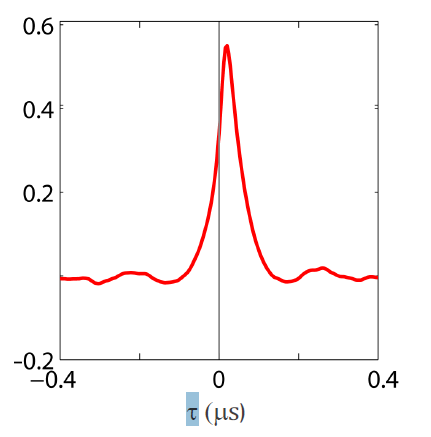
\includegraphics[scale=0.65]{Figures Cours Traitement du Signal/Cross-correlation function.png}
        \caption{Example of cross-correlation function}
        \label{fig:example_cross-correlation_function}
    \end{minipage}
\end{figure}

Compléter la suite après avoir compris.  
\newpage

\subsubsection{Auto-correlation}

If we consider \(y_2 = y_1 = y\), the cross-correlation (\ref{correlation function}) becomes the auto-correlation function :

\begin{equation}
    R_{xx}(\tau) = \frac{\sum_{i=0}^{N-\tau-1}(y_i - \overline{y})(y_{i+\tau}-\overline{y})}{\sigma_y ^2}
\end{equation}


\subsection{Statistical methods}

\subsubsection{Random variables and Probability Distribution Function (or PDF)}

First, we introduce the Cumulative Distribution Function which measures the probability that the variable \(x\) takes a smaller value than \(\alpha\) a number : 

\begin{gather*}
    F_x(\alpha) = P[x \leq \alpha]
\end{gather*}

The probability Density Function is related to CTDF as : 
\begin{equation*}
    f_x (\alpha) = \frac{\textrm{d}F_x (\alpha)}{\textrm{d}\alpha} ~~~~ F_x (\alpha) = \int_{-\infty}^{\alpha}f_x(x) \textrm{d}x
\end{equation*}

\newpage
\subsubsection{How to compute PDF in practice with discrete data ?}

\begin{figure}[h]
\begin{minipage}{0.5\textwidth}
   \paragraph{}
    It consists in dividing signal into bins and to count the number of samples in each bin which takes a value inferio or equal to \(\alpha\). The ideal number of bins is \(\sqrt{N}\), it is the one which provides best statistics. 

\paragraph{}
As a Probability Distribution Function, the function have also to be normalised : 

\begin{equation*}
    \int_{-\infty} ^{+\infty} f_x (x) \textrm{d}x = 1 
\end{equation*}
\end{minipage}
\begin{minipage}{0.5\textwidth}
    \centering
    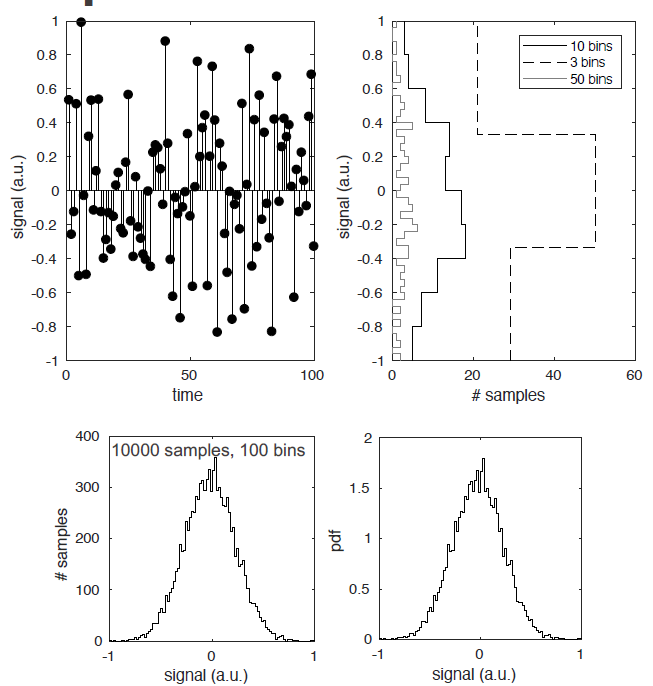
\includegraphics[scale=0.4]{Figures Cours Traitement du Signal/PDF in practice from discrete data.png}
    \caption{Construction of Probability Distribution Function}
    \label{fig:PDF}
\end{minipage}
\end{figure}

\subsubsection{Moments of the PDF}

\paragraph{Mean :}
\begin{equation}
    \overline{x} = \frac{1}{N} \sum_{j=0}^{N-1} x_j
\end{equation}

\paragraph{Variance :}

\begin{equation}
    \sigma^2 = \frac{1}{N-1} \sum_{j=0} ^{N-1} (x_j - \overline{x})^2
\end{equation}

\paragraph{Skewness :}
Third order moment, it "measures" the asymetry of the data around the samples mean. The skewness of the normal distribution (or any perfectly symetric distribution) is zero. 

\begin{equation}
    sk= \frac{1}{N} \sum_{j=0} ^{N-1} \left[\frac{x_j-\overline{x}}{\sigma}\right]^3
\end{equation}

\paragraph{Kurtosis (or Flatness) :}
Fourth order moment, it "measures" the peaking of the PDF with respect to the normal distribution. Kurtosis is a measure of how outlier-prone a distribution is. The kurtosis of normal distribution is 0. 

\begin{equation}
    kur = \frac{1}{N}\sum_{j=0}^{N-1}\left[\frac{x_j - \overline{x}}{\sigma}\right]^4-3
\end{equation}

\paragraph{Interest :}
The idea is to compare a data set to a known distribution or to compare two or more data sets distributions in order to get informations on physical process behind the data. 

\paragraph{}
The most commonly accepted test for comparing different binned PDFs is the Chi-squared test. 

\begin{equation}
    \chi^2 = \frac{1}{N=1}\sum_{j=0}^{N-1} (x_{exp} - x_{th})^2
\end{equation}

\subsubsection{PLASMAS}

\subsubsection{How to extract coherent structures : conditionnal averaging}

\paragraph{}
A signal can be decomposed with a time-dependent part and a fluctuating part : \(y(x,t) = \overline{y}(x) + \Tilde{y}(x,t)\)

\paragraph{}
The fluctuating part can be decomposed with a \textbf{coherent} part and a \textbf{random} one : \(y(x,t) = \overline{y} (x) + \tilde{y}_{coh} (x,t) + \tilde{y}_{rand}(x,t)\). An ensemble average over a lot of independent realization will remove the random part :

\begin{gather*}
    \langle \tilde{y}(x,t) \rangle = \langle \tilde{y}_{coh}(x,t) + \tilde{y}_{rand}(x,t) \rangle = \langle \tilde{y}_{coh}(x,t) \rangle + \langle \tilde{y}_{rand}(x,t) \rangle = \langle \tilde{y}_{coh}(x,t) \rangle 
\end{gather*}

\subsubsection{How to build an ensemble of independent realizations ?}

\begin{figure}[h]
    \begin{minipage}{0.5\textwidth}
        \paragraph{}
        The first step is to select a criterion : \(y_0 < y < y_0 + \Delta y_0\). Then, we have to select a time window : \(t_i - \Delta t < t < t_i + \Delta t \) where \(\Delta t\) is of the order of autocorellation time. 

        \paragraph{}
        The ensemble of independent realizations is obtained when the same time windows are identified in other signals. 
    \end{minipage}
    \begin{minipage}{0.5\textwidth}
    \centering
    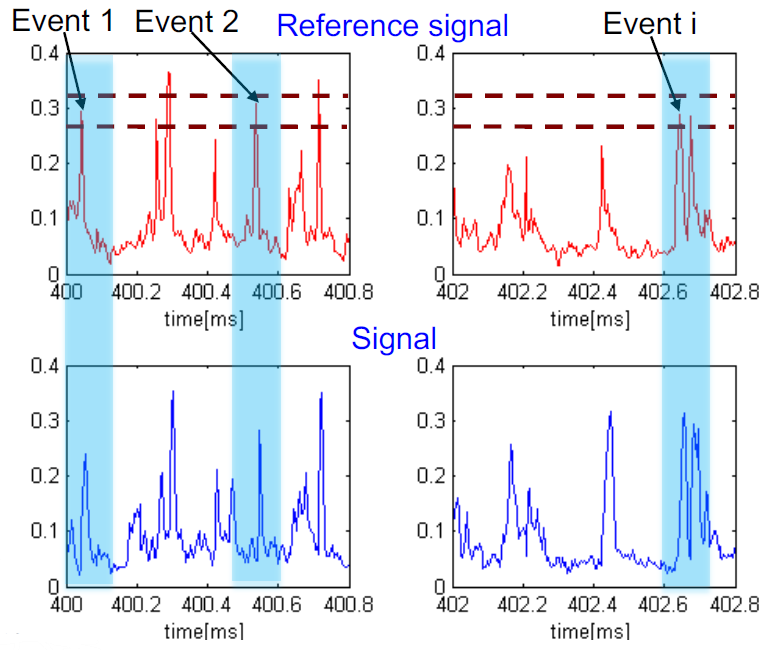
\includegraphics[scale=0.4]{Figures Cours Traitement du Signal/How to build independent realizations.png}
    \caption{}
    \label{fig:how to build an ensemble of independent realizations}
    \end{minipage}
\end{figure}

\subsubsection{Conditionnal averaging}

We Consider two signals : a reference signal and a "useful" signal. The figures \ref{fig:conditionnal averaging} is get when identified time windows are put together for the reference signal and the "useful" signal. 

\begin{figure}[h]
    \begin{minipage}{0.5\textwidth}
        \centering
        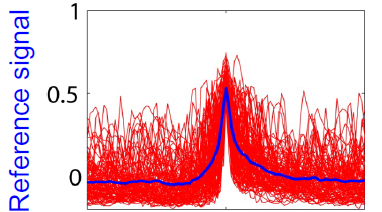
\includegraphics[scale=0.8]{Figures Cours Traitement du Signal/Reference signal 1.png}
    \end{minipage}
    \begin{minipage}{0.5\textwidth}
        \centering
        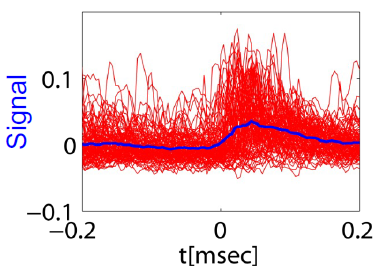
\includegraphics[scale=0.8]{Figures Cours Traitement du Signal/Useful Signal - 2.png}
    \end{minipage}
    \caption{}
    \label{fig:conditionnal averaging}
\end{figure}

\paragraph{}
The maxima in the average reference signal and in the average "useful" signal are not reached at the same time. 

\newpage
\subsubsection{Conditional averaging allows reconstructing 2D/3D
dynamics}

\begin{figure}[h]
    \begin{minipage}{0.5\textwidth}
        \paragraph{}
        The red probe is the reference probe, fixed and detecting an event. The blue probe ("useful" probe) is moved between two shots over the green area to sample 2D dynamics of a coherent event. It can measure a different quantity from the reference probe.

        \paragraph{IMPORTANT :} 
        The signals have to be stationary to shot-to-shot reproductibility. 
    \end{minipage}
    \begin{minipage}{0.5\textwidth}
        \centering
        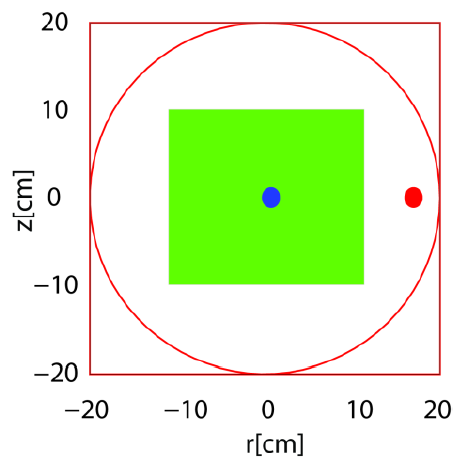
\includegraphics[scale=0.4]{Figures Cours Traitement du Signal/2D 3D.png}
        \caption{Representation of both probes}
        \label{fig:2D/3D synamics}
    \end{minipage}
    
\end{figure}

\newpage
\printbibliography

\end{document}

